\Chapter{Die MMU}
\label{ch:mmu}

Die MMU (Memory Management Unit) verwaltet den in Bl\"ocke gegliederten Speicherbereich und die darauf erfolgenden Zugriffe. Die Einheit bietet dabei eine Schnittstelle für lesende und schreibende Speicheranfragen, welche in unterschiedlichen Zeitintervallen bearbeitet werden.

\Section{\"Uberblick}

Der adressierbare Speicher innerhalb des Prozessors ist blockweise organisiert. Die MMU verwaltet einerseits die einzelnen Controller für die jeweiligen RAM-Bl\"ocke und taktet andererseits die angefragten Zugriffe auf diese.

Sie ist aufgrund der \"uberwiegend sehr \"ahnlichen Adressierungsprozeduren intern durch eine Statemachine realisiert, welche anhand einer Speicheradresse die jeweiligen Speicheranfragen an den dem RAM-Block entsprechenden Controller weiterleitet.

Um eine reibungslose Kommunikation mit diesen Controllern zu gew\"ahrleisten, ist die MMU mit einer vom restlichen Prozessor unterschiedlichen Frequenz, 133 MHz, getaktet. Dies ist vor allem im Bezug auf den integrierten DDR2-SDRAM\footnote{Genauer handelt es sich um einen Micron Technology DDR2-SDRAM (MT47H32M1)}, welcher mit eben diesem Takt versorgt werden muss, um Daten halten zu k\"onnen, begr\"undet: Die Tatsache, dass die Integration dieser Komponente besonders zeitaufw\"andig verlief, rechtfertigt diese Designentscheidung. Daraus resultieren zus\"atzlich ben\"otigte Synchronisations- und Kommunkationsmechanismen mit dem \"ubergeordneten Leitwerk.
\newpage
\Section{Interface}
Das Interface der MMU untergliedert sich haupts\"achlich in drei verschiedene Komponenten: Einerseits Signale zur Kommunikation mit dem Leitwerk, andererseits durch das Toplevel-Modul nach oben geleitete Signale zur Adressierung des DDR2-SDRAMs, welche vom in der MMU verwalteten Controller generiert werden, und zuletzt nach oben geleitete Daten- und Adressleitungen, die die ASCII-Einheit konstant mit Daten versorgt.

\begin{figure}[H]
	\centering
		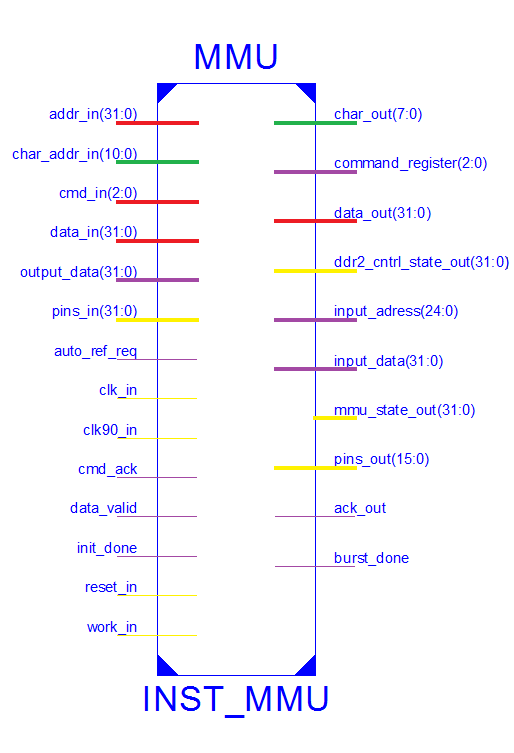
\includegraphics[width=0.5\textwidth]{interface.png}
	\caption{Schnittstelle der MMU-Einheit, Signale farblich gruppiert: \textit{Rot} = Kommunikation mit Leitwerk, \textit{Gr\"un} = Character-Ausgabe an ASCII-Einheit, \textit{Violett} = Verbindung mit DDR2-SDRAM, \textit{Gelb} = Sonstige}
	\label{fig:mmuinterface}
\end{figure}

\Subsection{Kommunikation mit dem Leitwerk}

Die Kommunikation mit dem Leitwerk l\"asst sich im Wesentlichen in Daten-, Adress- und Synchronisationsleitungen untergliedern. Dabei sendet das Leitwerk \"uber das Signal cmd\_in die angefragte Operation. Die MMU reagiert allerdings erst auf ein Setzen des work\_in Signals mit der Bearbeitung der Anfrage. Der 3-Bit Vektor cmd\_in ist wie folgt aufgebaut:

\begin{center}
	\begin{tabular}{| l | l |}
		\hline
		Bit 2 & 1 Bit 1 - 0 \\ \hline
		0 := Read, 1 := Write & 0 := 8 Bit, 1 := 16 Bit, 3 := 32 Bit \\ 		\hline
	\end{tabular}
\end{center}

Als Ausgabe liefert die MMU dem Leitwerk einerseits ein Acknowledgement ack\_out, welches signalisiert, dass die MMU bereit ist, eine neue Anfrage zu bearbeiten und indirekt damit auch Auskunft dar\"uber gibt, ob die bereits gesendete Anfrage erfolgreich bearbeitet wurde. Im Falle eines lesenden Speicherzugriffs wird, sofern das Acknowledgement-Signal den Wert 1 angenommen hat, gew\"ahrleistet, dass der Datenausgang data\_out korrekt belegt wurde.

Es sei angemerkt, dass w\"ahrend im Zuge der Entwicklung und der stark \"uberwiegenden Zahl der 32-Bit Lesezugriffe (vor allem im Zuge des Ladens eines Befehls) beschlossen wurde, dass jeder lesende Speicherzugriff ungeachtet der im cmd\_in definierten Datenbreite 32-Bit  lie\ss{}t. Theoretisch bietet die MMU allerdings auch die M\"oglichkeit, 8-Bit oder 16-Bit Lesezugriffe durchzuf\"uhren.

\Subsection{Durch die MMU geleitete Signale an andere Komponenten}

Wie eingangs erw\"ahnt lassen sich die \"ubrigen Signale dem Weiterleiten von Signalen aus einerseits dem Controller der DDR2-SDRAM-Komponente sowie den kontinuierlichen lesenden Anfragen der ASCII-Einheit an den entsprechenden CHARRAM-Block (die parallel und unabh\"angig von der Funktionalit\"at der MMU laufen) zuordnen und werden hier nicht weiter vertieft.

\Section{Aufbau des Speichers}

Wie bereits geschildert wird der Speicher in verschiedene Bereiche unterschiedlicher Gr\"o\ss{}e untergliedert. Jeder dieser Bereiche wird von einem Controller verwaltet, welcher bei einer eingehenden Anfrage durch die MMU angesprochen wird. Dabei h\"angt die Bearbeitungsdauer ma\ss{}geblich vom adressierten Speicherblock ab.

Aus der durch den Prozessor implementierten Wortgr\"o\ss{}e von 32 Bit ergibt sich ein Adressraum, potenziell $2^{32}$ potenzielle Speicherzellen mit einer Gr\"o\ss{}e von je 8 Bit umfasst. Dass nicht jeder dadurch zur Verf\"ugung stehende Bereich auch tats\"achlich auch nutzbar ist, l\"asst sich auf die vom FPGA zur Verf\"ugung gestellten Speicherressourcen zur\"uckf\"uhren.

Stattdessen wird die Adresse in ein Pr\"afix, welches den adressierten Speicherbereich bestimmt, und ein Offset innerhalb dieses Speicherblocks wie folgt unterteilt:

\begin{center}
	\begin{tabular}{| l | l |}
		\hline
		Bit 31 - 28 & Bit 27 - 0 \\ \hline
		Pr\"afix & Offset \\ \hline
	\end{tabular}
\end{center}

Insgesamt existieren f\"unf zul\"assige Werte f\"ur das 4-Bit Pr\"afix, wobei Zugriffe auf nicht g\"ultige Speicherpr\"afixe nicht verarbeitet werden. Zudem unterscheiden sich die Gr\"o\ss{}en der jeweiligen Speicherbl\"ocke von dem potenziell 28-Bit gro\ss{}en Raum innerhalb eines Blocks. Aufgrund der Tatsache aber, dass diese sich stets als nat\"urliche Potenz von 2 darstellen lassen, kann durch Spiegelung des tats\"achlich nutzbaren Speicherraums der gesamte vom Offset darstellbare Bereich adressiert werden. Im Endeffekt wird der Offset also lediglich in seiner wirksamen Gr\"o\ss{}e entsprechend des Speicherblocks beschnitten. Die folgende Tabelle zeigt die implementierten Speicherbl\"ocke sowie deren nutzbare Gr\"o\ss{}e.

\begin{table}[h]
	\begin{center}
	\begin{tabular}{| l | l | l | l |}
		\hline
		Pr\"afix & K\"urzel & Gr\"o\ss{}e in Bytes & Kurzbeschreibung \\ \hline
		0x0 & BIOS & $2^{11}$ & Programmeinsprungspunkt \\ \hline
		0x1 & SDRAM & $2^{16}$\footnote{Von 512 MBit verf\"ugbaren Speicherplatz macht der genutzte Controller nur $2^{16}$ Bytes zug\"anglich} & DDR2-SDRAM \\ \hline
		0x2 & CHARRAM & $2^{11}$ & Character-Anzeige \\ \hline
		0x3 & IORAM & $2^{3}$ & Memory-Mapped I/O \\ \hline
		0x4 & SERIALRAM & $2^{11}$ & Serielle Schnittstelle \\ \hline
	\end{tabular}
	\end{center}
	\label{tab:ramlayout}
\end{table}

Dabei sind alle Bl\"ocke, ausgenommen der DDR2-SDRAM-Block, durch auf dem FPGA verf\"ugbaren Dual-Port-Blockram realisiert, sodass die implementierten Controller im Groben gleich sind. Angemerkt sei an dieser Stelle, dass - in Absprache mit dem Betreuer - der Controller f\"ur den DDR2-SDRAM eine Implementierung von \href{http://opencores.org/project,ddr2_sdram}{Opencores}\footnote{\url{http://opencores.org/project,ddr2_sdram}} verwendet und entsprechend den Anforderungen abge\"andert.

Jeder Speicherbereich wird von der MMU im Little-Endian-Format adressiert, was insbesondere bei 16-Bit beziehungsweise 32-Bit Zugriffen ber\"ucksichtigt werden muss.

\Section{Memory-Mapped I/O}
\label{sec:mmuio}
Einer der geschilderten Speicherbl\"ocke, genauer der IORAM, stellt die Schnittstelle zwischen Benutzer und Programmcode dar. Dabei sind einige der auf dem FPGA verf\"ugbaren Ein- und Ausgabem\"oglichkeiten direkt auf einzelne Bits innerhalb der Speicherzellen des IORAMs gemappt. Aus den acht verf\"ugbaren Speicherzellen sind folgende sechs nutzbar:

\begin{center}
	\begin{tabular}{| c | c | c | c | c | c | c | c | c | c |}
	\hline
	Zelle & R/W & Bit 7 & Bit 6 & Bit 5 & Bit 4 & Bit 3 & Bit 2 & Bit 1 & Bit 0 \\ \hline
	0x0 & Read-Only & BTN 0 & - & - & - & - & - & - & - \\ \hline
	0x1 & Read-Only & SW 3 & SW 2 & SW 1 & SW 0 & BTN 4 & BTN 3 & BTN 2 & BTN 1 \\ \hline
	0x2 & Read/Write & LED 7 & LED 6 & LED 5 & LED 4 & LED 3 & LED 2 & LED 1 & LED 0 \\ \hline
	0x3 & Read/Write & - & - & - & - & - & - & - & - \\ \hline
	0x4 & Read-Only & UART 7 & UART 6 & UART 5 & UART 4 & UART 3 & UART 2 & UART 1 & UART 0 \\ \hline
	0x5 & Read-Only & - & - & - & - & - & - & UART VALID & UART ERR \\ \hline
	0x6 & Read/Write & - & - & - & - & - & - & - & - \\ \hline
	0x7 & Read/Write & - & - & - & - & - & - & - & - \\ \hline
	\end{tabular}
\end{center}

Dabei steht BTN jeweils f\"ur entsprechende Buttons auf dem Board, SW entspricht einem Schalter und LED den Ausgabe-LEDs. Au\ss{}erdem sind die Eingabedaten der seriellen Schnittstelle in Form eines 8-Bit Vektors sowie einem Best\"atigungssignal, dass dieser vollst\"andig \"ubertragen wurde und einem Fehlersignal, das ebenfalls von der seriellen Schnittstelle ausgeht, ebenfalls auf den IORAM gemappt. Angemerkt sei an dieser Stelle aber, dass der Prozessor nicht schnell genug taktet, um diese Funktionalit\"at wirklich sinnvoll zu nutzen, weswegen zur Initialisierung des Programmspeichers auch eine andere Methode verwendet wird. Bits, die nicht genutzt und in der Tabelle mit - vermerkt sind, entsprechen stets dem konstanten Wert 0 und bieten daher auch keinerlei Speicherqualit\"at.

Die nachfolgende Abbildung~\ref{fig:pinning} zeigt, wo sich welches Ein-/Ausgabesignal auf der Hardware wiederfindet. Dabei entsprechen die Bezeichner denen aus der zuvor abgebildeten Tabelle.

\begin{figure}[H]
	\centering
		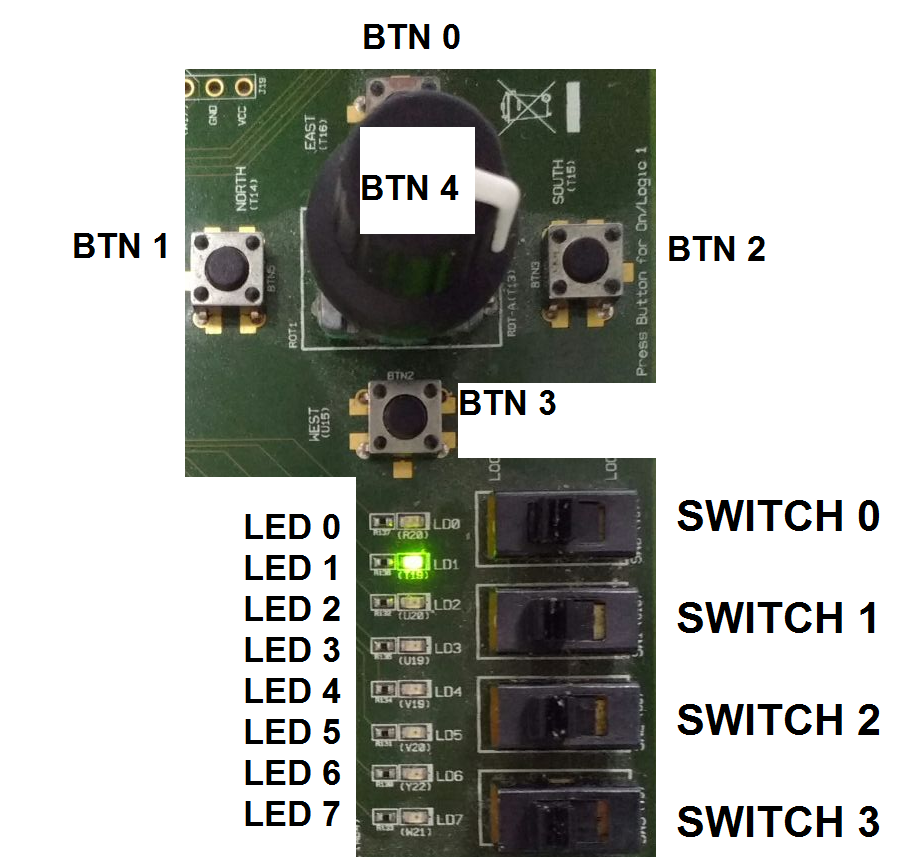
\includegraphics[width=0.5\textwidth]{pinning.png}
	\caption{Verteilung der I/O-Signale}
	\label{fig:pinning}
\end{figure}


\Section{Implementierung als State Machine}

Aufgrund der identisch aufgebauten Controller f\"ur die meisten Speicherbl\"ocke ist die MMU durch eine State Machine realisiert. Dabei die MMU zwar im State MMU-IDLE initialisiert, wechselt bei einem Reset den Zustand aber sofort zu MMU-RESET.

Das nachfolgende Zustands\"ubergangsdiagramm veranschaulicht die durch einen Lese- oder Schreibzugriff entstehende Prozedur.

\Statemachine{./mmu/mmu_state.pdf}{
Zustands\"ubergangsdiagramm der MMU. \"Uberg\"ange zum Zustand \textbf{MMU-RESET}, die von jedem anderen Zustand durch \Vhdl{rst\_in = '1'} ausgel\"ost werden, sind der \"Ubersicht halber ausgelassen.
}

\Subsection{MMU-IDLE}

Im Zustand MMU-IDLE wartet die Einheit auf das eingehen eines Befehls \"uber das \Vhdl{cmd\_in} Signal. Solange dies nicht erfolgt, wird das Synchronisationssignal \Vhdl{ack\_out} mit dem Wert 1 belegt. Anderenfalls wird die Eingabeadresse ausgewertet, die durchzuf\"uhrende Operation an den entsprechenden RAM-Controller weitergeleitet und die Einheit in den Zustand MMU-WAITING \"uberf\"uhrt.

\Subsection{MMU-WAITING}

Durch diesen Zustand wird die Ausf\"uhrung eines Lese- oder Schreibzugriffs solange verz\"ogert, bis der entsprechende RAM-Controller die 8-Bit Anfrage erfolgreich bearbeitet hat. Im Fall des DDR2-SDRAM-Controllers erfolgt dies \"uber ein Synchronisationssignal, anderenfalls kann mit einer festen Wartedauer von einem Takt gerechnet werden. W\"ahrend des Wartevorgangs werden die Befehle, die am entsprechenden RAM-Controller anliegen, entfernt.

Sollte der Controller bereit sein, eine neue 8-Bit Anfrage zu verarbeiten, wird die MMU in den Zustand MMU-DATA-VALID \"uberf\"uhrt.

\Subsection{MMU-DATA-VALID}
In diesem Zustand werden, sofern es sich bei der zuletzt durchgef\"uhrten Operation um einen Lesezugriff gehandelt hat, die gelesenen Daten mittels eines Buffer-Signals zwischengespeichert. Au\ss{}erdem wird die Einheit je nach Zugriffsmodus in den Zustand MMU-READ-NEXT beziehungsweise MMU-WRITE-NEXT \"uberf\"uhrt.

\Subsection{MMU-READ-NEXT}

Sofern noch weitere 8-Bit Zellen gelesen werden m\"ussen, wird eine neue lesende Anfrage an den entsprechenden RAM-Controller weitergeleitet und  die Einheit wieder in den Zustand MMU-WAITING \"uberf\"uhrt. Anderenfalls wechselt die MMU in den Zustand MMU-READ-DONE.

\Subsection{MMU-READ-DONE}

Alle gelesenen und zwischengespeicherten Daten werden gem\"a\ss{} dem Little-Endian-Encoding zusammengesetzt und auf der Datenausgabeleitung an das Leitwerk \"ubergeben. Damit einher geht das Setzen des Acknowledgements-Signals \Vhdl{ack\_out} auf den Wert 1 sowie der Zustandswechsel nach MMU-IDLE.

\Subsection{MMU-WRITE-NEXT}

Sollte der vom Leitwerk geforderte Schreibzugriff weitere schreibende 8-Bit Zugriffe erfordern, wird in diesem Zustand der der Adresse entsprechende RAM-Controller mit neuen Daten und einer inkrementierten Adresse angesprochen und die MMU-Einheit in den Zustand MMU-WAITING \"uberf\"uhrt. Anderenfalls wechselt die MMU in den Zustand MMU-WRITE-DONE.

\Subsection{MMU-WRITE-DONE}

Da nach einem erfolgreichen Schreibzugriff keinerlei Ausgabedaten \"ubermittelt werden m\"ussen, wird in diesem Zustand lediglich das Acknowledgement-Signals \Vhdl{ack\_out} auf den Wert 1 gesetzt sowie die Einheit zur\"uck in den Zustand MMU-IDLE \"uberf\"uhrt.

\Subsection{MMU-RESET}

Bei einem Reset wechselt die MMU ungeachtet ihres derzeitigen Zustands in den MMU-RESET Zustand und unterbricht alle derzeitigen Anfragen ausnahmslos. Da die Einheit das eingehende Reset-Signal an alle RAM-Controller weitergeleitet, wird in diesem Zustand lediglich auf  die Beendigung der Resets jedes einzelnen Controllers gewartet. Sollten diese wieder bereit f\"ur neue Anfragen sein, wechselt die MMU wieder in den MMU-IDLE Zustand.

\Section{Zugrifssdauer}

Aus dem geschilderten detaillierten Ablauf eines Zugriffs innerhalb der MMU lassen sich nun f\"ur die einzelnen Speicherbl\"ocke die exakten Zugriffsdauern beziehungsweise im Fall des DDR2-SDRAMs, welcher unter Umst\"anden durch einen periodisch auftretenden Auto-Refresh eine erh\"ohte Zugriffszeit ben\"ontigt, eine Mindestzugriffsdauer errechnen.

\begin{center}
	\begin{tabular}{| l | l | l | l |}
		\hline
		Datengr\"o\ss{}e & (minimale) Zugriffsdauer \\ \hline
		8-Bit & 4 Takte \\ \hline 
		16-Bit & 7 Takte \\ \hline
		32-Bit & 13 Takte \\ \hline
	\end{tabular}
\end{center}

Aufgrund der identischen Struktur der RAM-Controller f\"ur als Dual-Port-Blockram realisierte Speicherbereiche ergeben sich f\"ur jene Speicherbl\"ocke identische Zugriffszeiten sowohl f\"ur lesende und schreibende Zugriffe, wobei eine 8-Bit Anfrage immer genau einen Takt kostet. Da der DDR2-SDRAM f\"ur seine Zugriffsdauer im Bezug auf lesende und schreibende Operationen nicht nach oben hin abgesch\"atzt werden kann, jedoch keinesfalls weniger als einen Takt brauchen wird, entsprechen die Mindestzugriffszeiten ebenfalls der oben dargestellten Tabelle.


